Alternativ kann man dies auch mit dem folgenden, von mir geschriebenen MATLAB Skript berechnen:
\begin{minted}{Matlab}
    %--- Zuerst die Matrizen definieren
    A=[1 2 0; 4 3 0; 0 0 1];
    B=[2 7 -2; 4 0 1; 1 4 0];
    C=[1 0 0 -1; -2 4 3 0];
    D=[1 1; 1 1; 0 2; 1 2];
    F=[4; 3; 1];
    G=[2 2 1];
    I=eye(3);
    
    %B, C und D transponieren
    BT=B.';
    CT=C.';
    DT=D.';
    
    % Teilaufgabe a)
    disp('Die Lösung der Teilaufgabe a) ist: ');
    a=3*A-2*BT+I;
    disp(a);
    
    % Teilaufgabe b)
    disp('Die Lösungen von b) sind: ');
    b1=(A+B)*F;
    b2=A*F+B*F;
    disp(b1);
    disp('und')
    disp(b2);
    
    % Teilaufgabe c)
    disp('Die Lösungen von c) sind: ');
    c1=G*F;
    c2=F*G;
    disp(c1);
    disp('und');
    disp(c2);
    
    % Teilaufgabe d)
    disp('Die Lösungen von d) sind: ');
    d1=C*D;
    d2=DT*CT;
    disp(d1);
    disp('und');
    disp(d2);  
\end{minted}

Die Ausgabe davon ist: \\

\begin{figure}
     \centering
     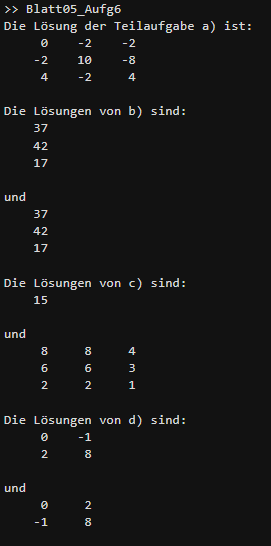
\includegraphics[width=0.5\textwidth]{Aufgaben/06/image.png}
     \caption{Ausgabe des Matlab Skriptes}
     \label{fig:enter-label}
 \end{figure}
